%%%%%%%%%%%%%%%%%%%%%%%%%%%%%%%%%%%%%%%%%%%%%%%%%%%%%%%%%%%%%%%%%%%%%%%%%%
%%%%%%%%%%%%%%%%%%%%%%%%%%%%%%%%%%%%%%%%%%%%%%%%%%%%%%%%%%%%%%%%%%%%%%%%%%
\clearpage{}
\section{Selection optimization - MVA}
\label{sec:MVA}
% ---- ---- ---- ---- ---- ---- ---- ---- ---- ---- ---- ---- ---- ---- ----

We have considered a multi-variate approach to further improve the signal and background separation in the analysis. It is performed by combining several observables into a Boosted Decision 
Trees (BDT) using the TMVA analysis package \cite{TMVA}. Two sets of BDT are used, depending on the purpose - search for $WW\gamma$ or aQGC signal. Additionally we do 
differentiation between muon and electron channels. That results in total of four BDTs. As a signal we use MC sample of SM $WW\gamma$ or aQGC with 
$a_{0}^{W}/\Lambda^{2}=-3.10^{5} GeV^{-2}$. As background are used MC $W\gamma+jets$ and data driven fake photon samples. Relative weight of those samples represent their 
contribution to the observed rate in the data. MC samples, used in the training of the BDTs also include per event pile-up and scale factors weights. Selection of the events 
follows the one described in section ~\ref{sec:reco}, with relaxed $m_{jj}$ cut to increase the statistics, needed for the BDT training process.

For the aQGC BDTs are used the following input variables:
\begin{itemize}
\item lepton transverse momentum 
\item missing transverse energy
\item transverse momentum of the leading central jet
\item transverse momentum of the next-to-leading central jet
\item sum of the transverse energy
\item distance between the two central jets in the $\eta-\phi$ plan
\item azimuthal angle between the two central jets
\item azimuthal angle between the photon and lepton
\item azimuthal angle between the photon and missing transverse energy
\item di-jet invariant mass.
\end{itemize}

Input variables distributions for aQGC BDT are shown in Figure~\ref{fig:InAQGCmu} for the muon channel. Distributions for electron channel are similar.

\begin{figure}[]
  \begin{center}
    \subfloat{
    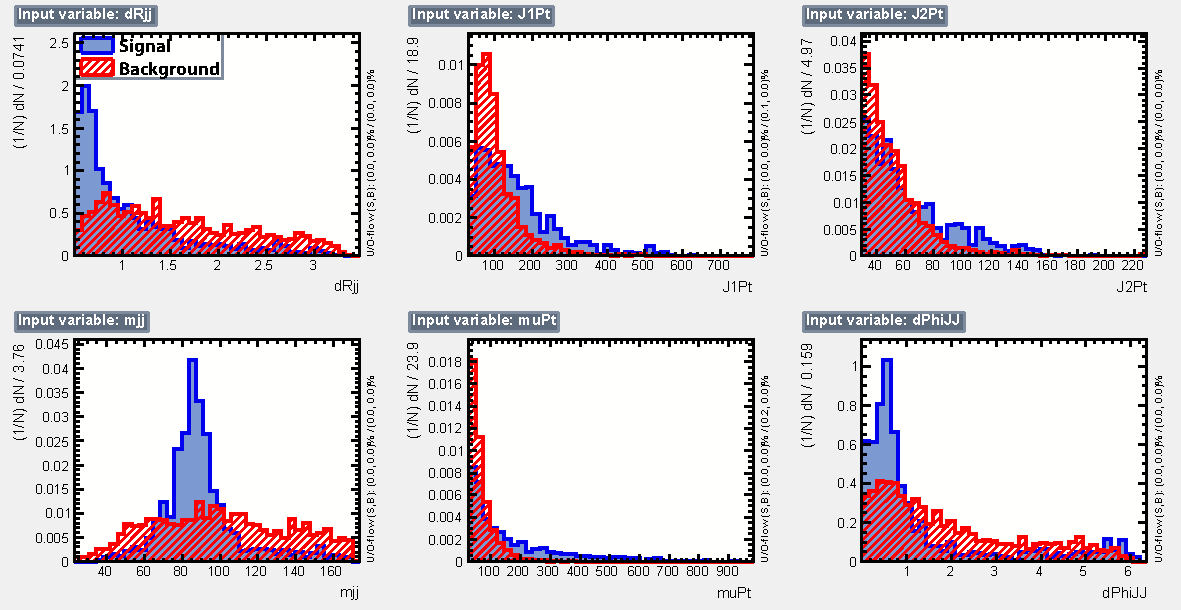
\includegraphics[width=0.9\textwidth]{figs/variables_aQGC_c1.pdf}
  }\\
  \subfloat{
    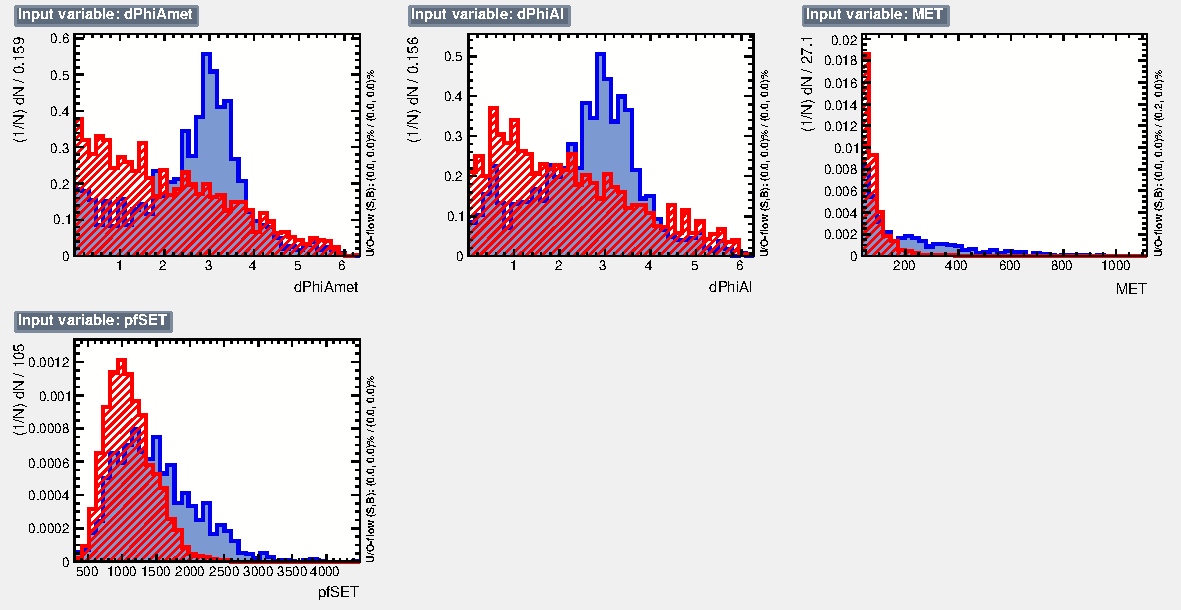
\includegraphics[width=0.9\textwidth]{figs/variables_aQGC_c2.pdf}
  }
    \caption{ Input variables distributions for aQGC BDT }
    \label{fig:InAQGCmu}
  \end{center}
\end{figure}

The linear correlations between the input variables for signal and background are shown in Figure~\ref{fig:corrAQGCmu} for aQGC BDT muon channel.

\begin{figure}[]
  \begin{center}
    \subfloat{
    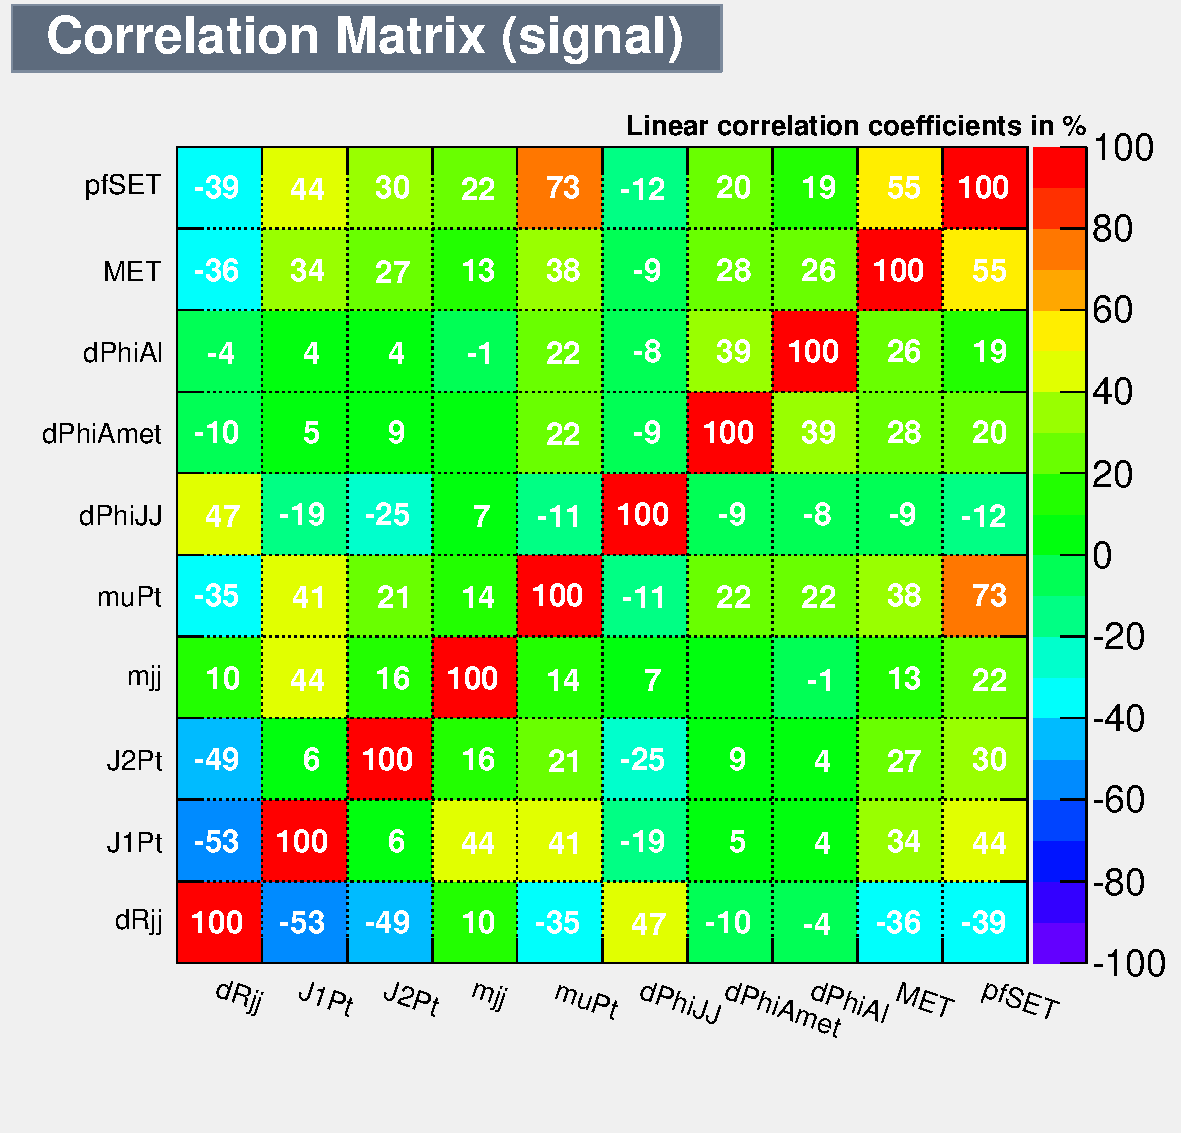
\includegraphics[width=0.4\textwidth]{figs/CorrelationMatrixS_aQGC.pdf}
  }
  \subfloat{
    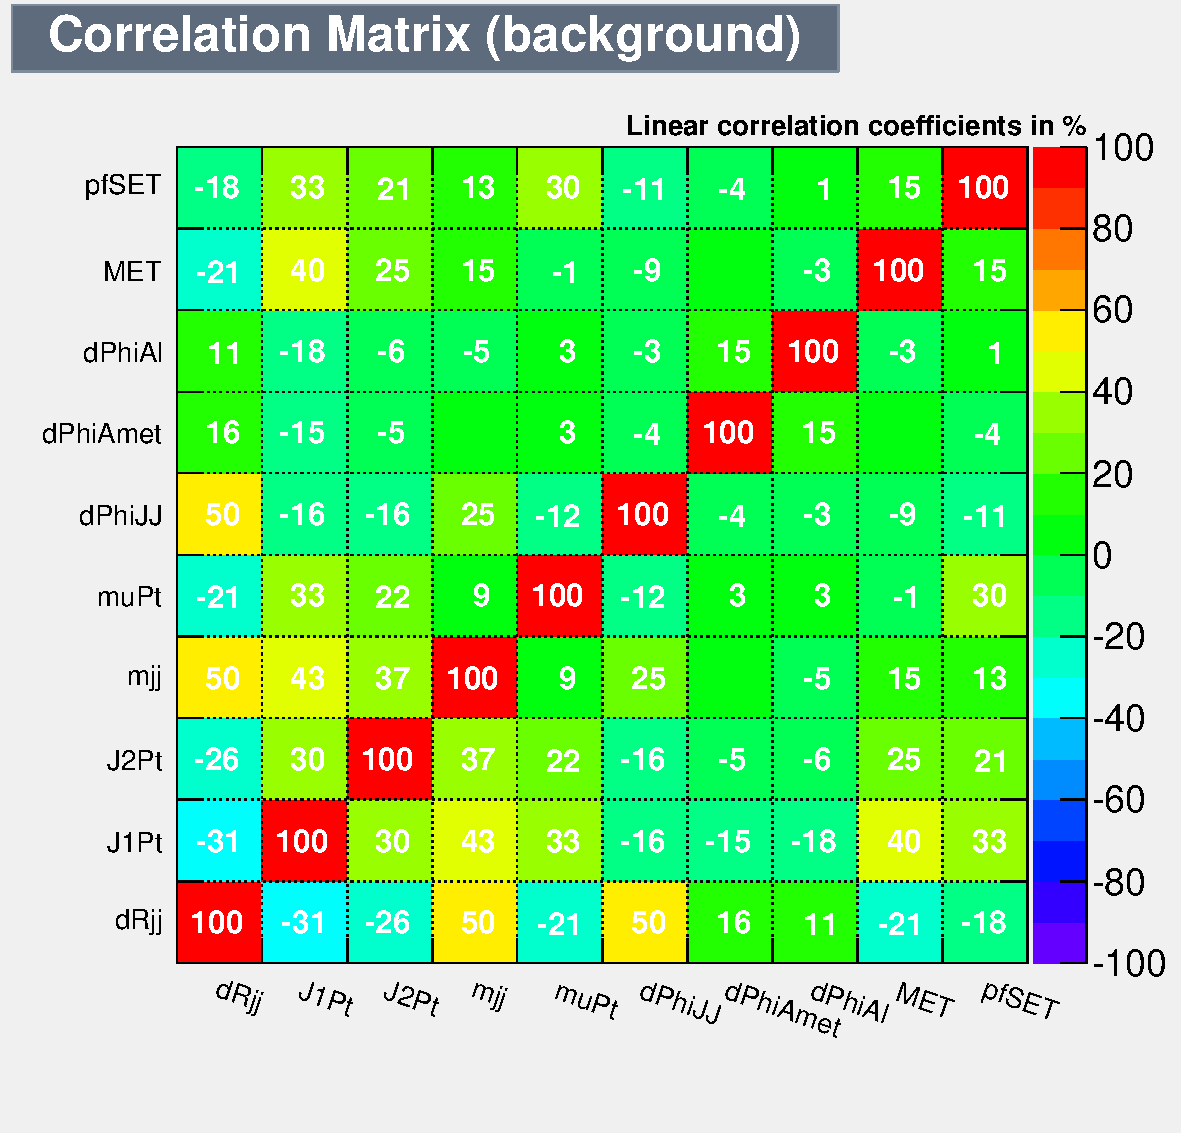
\includegraphics[width=0.4\textwidth]{figs/CorrelationMatrixB_aQGC.pdf}
  }
    \caption{ The linear correlations between the input variables for signal and background for aQGC BDT muon channel. }
    \label{fig:corrAQGCmu}
  \end{center}
\end{figure}

The data-MC comparison for the aQGC MVA output is shown on Figure ~\ref{fig:outaQGCmu}

\begin{figure}[b]
  \begin{center}
    \subfigure[]{
    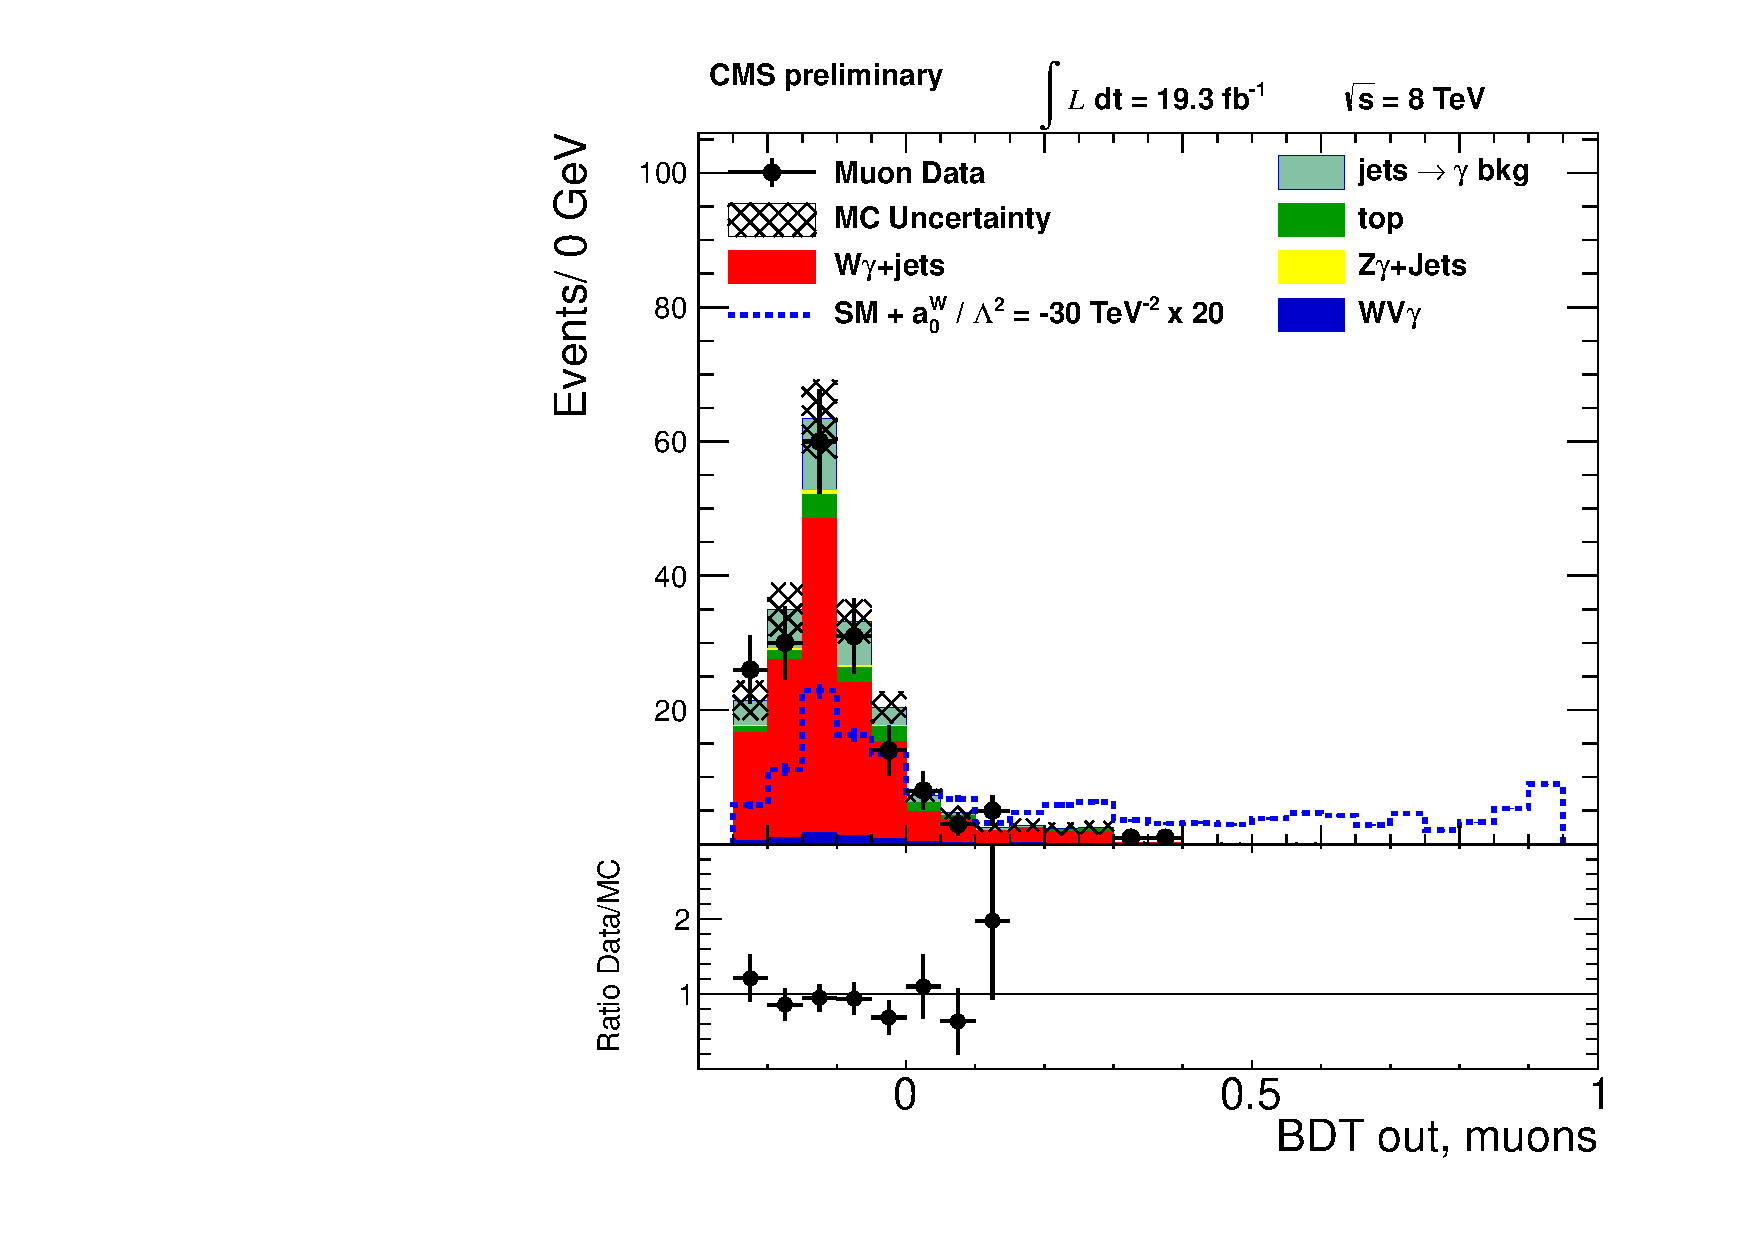
\includegraphics[width=0.4\textwidth]{figs/mu_mva2jWWAmuA11.pdf}
  }
  \subfigure[]{
    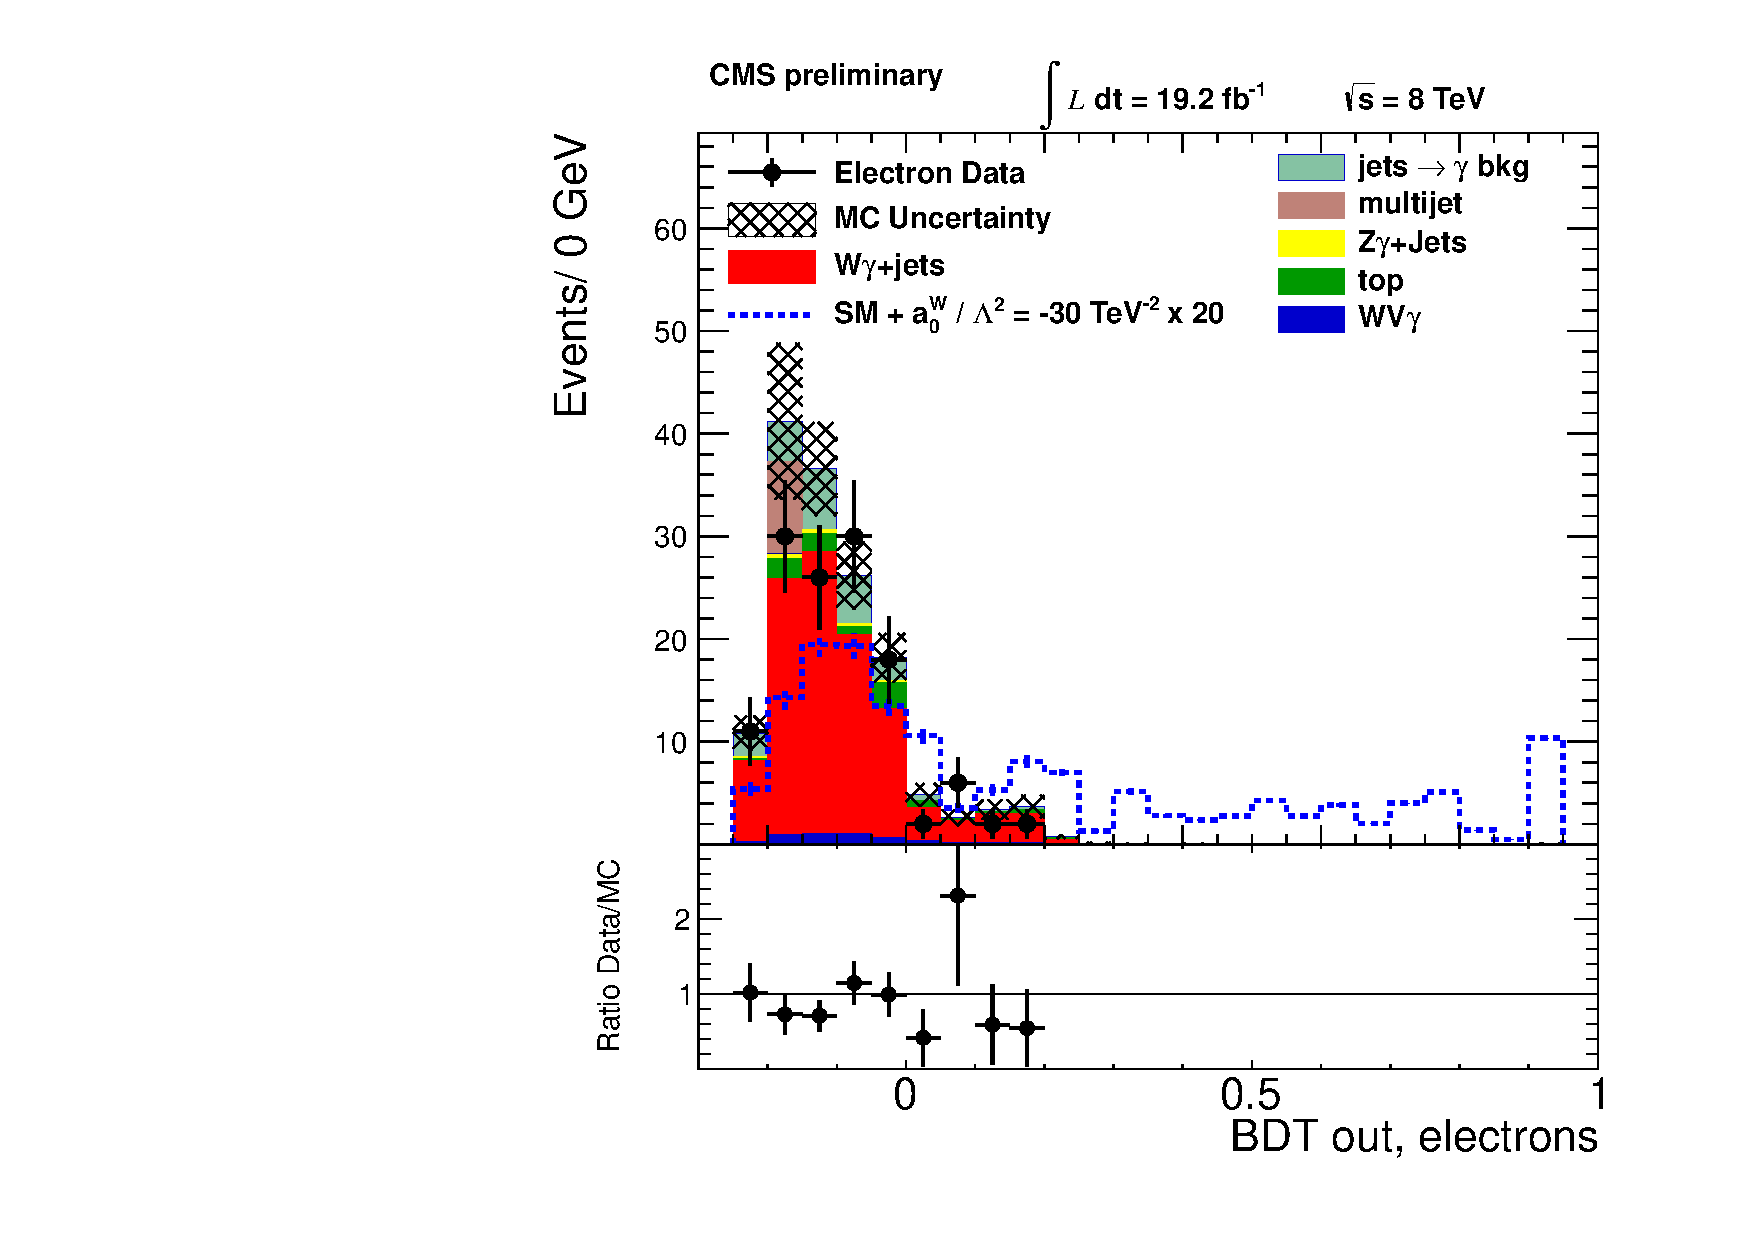
\includegraphics[width=0.4\textwidth]{figs/el_mva2jWWAelA11.pdf}
  }
    \caption{ Data-MC comparison for the aQGC MVA output of (a) muon and (b) electron channel. }
    \label{fig:outaQGCmu}
  \end{center}
\end{figure}

 The cut value on the MVA output is chosen in a way that it keeps very high signal efficiency for events with high photon pT, while provides modest background 
rejections (in the range 30-50%). The singal efficiency is 98$\%$ (97$\%$) for signal events with photon pT larger than 300 GeV(200 GeV).

 
For the SM $WW\gamma$ BDTs are used the following input variables:
\begin{itemize}
\item transverse momentum of the leptonic W
\item distance between the two central jets in the $\eta-\phi$ plan
\item transverse momentum of the leading central jet
\item transverse momentum of the next-to-leading central jet
\item di-jet invariant mass.
\item invariant mass of the $l,\nu,j,j,\gamma$ system
\item transverse momentum of the $l,\nu,j,j,\gamma$ system
\end{itemize}

Input variables distributions for SM $WW\gamma$ BDT are shown in Figure~\ref{fig:InSMmu} for the muon channel. Distributions for electron channel are similar.

\begin{figure}[]
  \begin{center}
    \subfloat{
    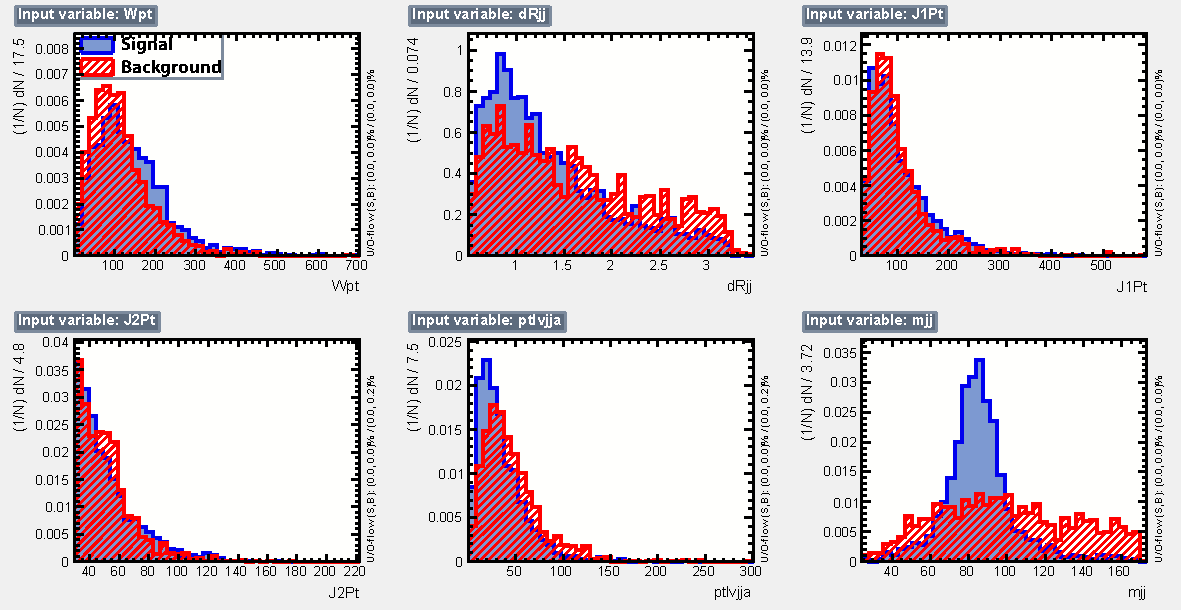
\includegraphics[width=0.9\textwidth]{figs/variables_SMWWA_c1.pdf}
  }\\
  \subfloat{
    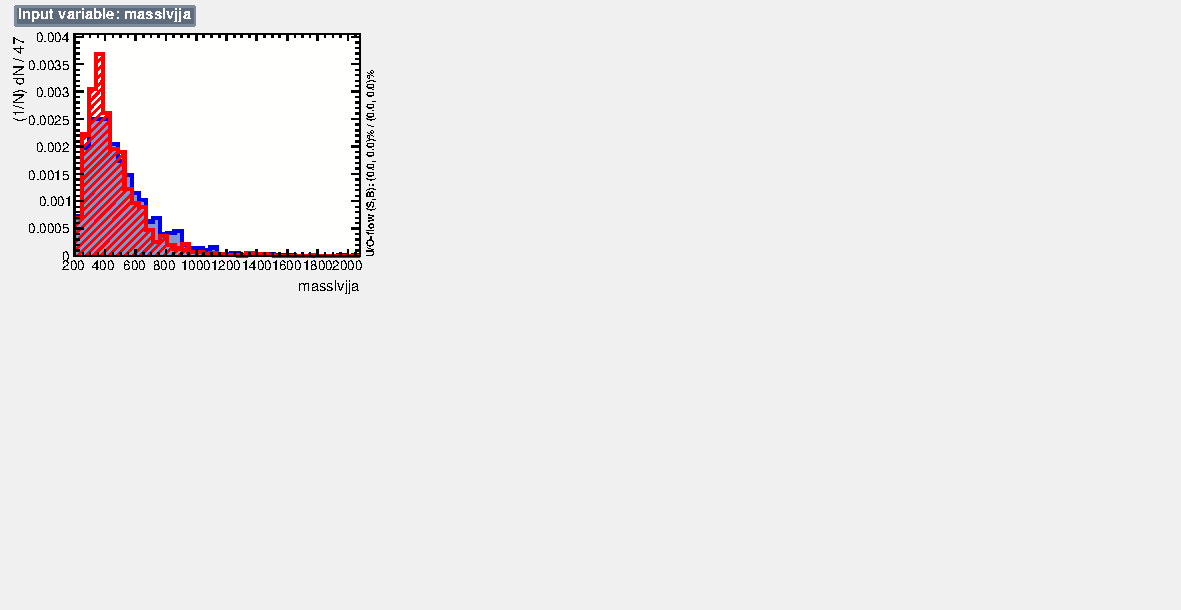
\includegraphics[width=0.9\textwidth]{figs/variables_SMWWA_c2.pdf}
  }
    \caption{ Input variables distributions for SM $WW\gamma$ BDT }
    \label{fig:InSMmu}
  \end{center}
\end{figure}

The linear correlations between the input variables for signal and background are shown in Figure~\ref{fig:corrSMmu} for SM $WW\gamma$ BDT muon channel.

\begin{figure}[]
  \begin{center}
    \subfloat{
    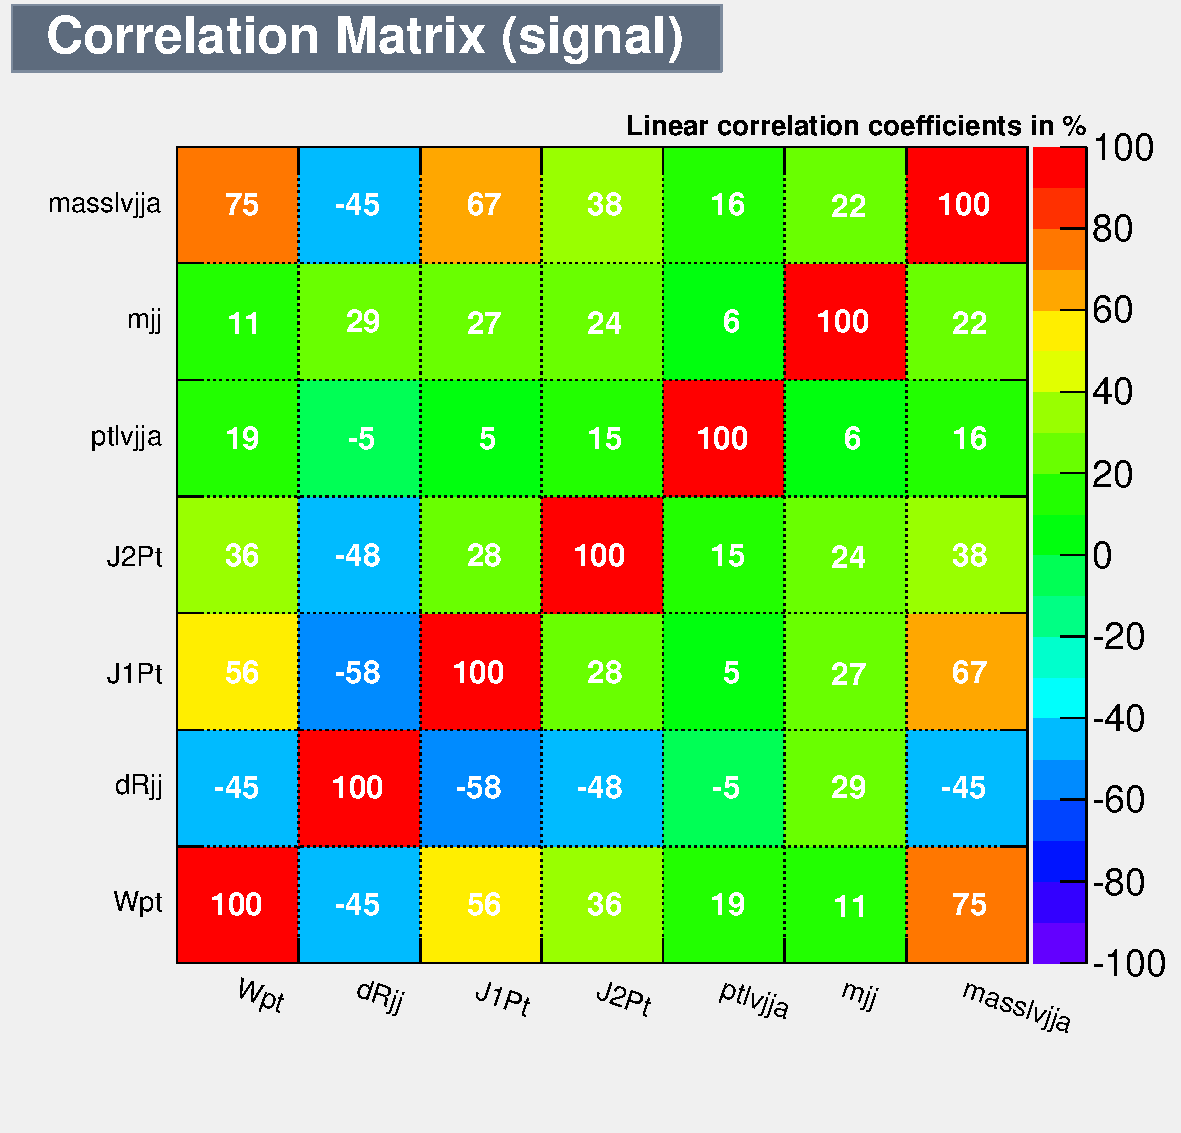
\includegraphics[width=0.4\textwidth]{figs/CorrelationMatrixS_SMWWA.pdf}
  }
  \subfloat{
    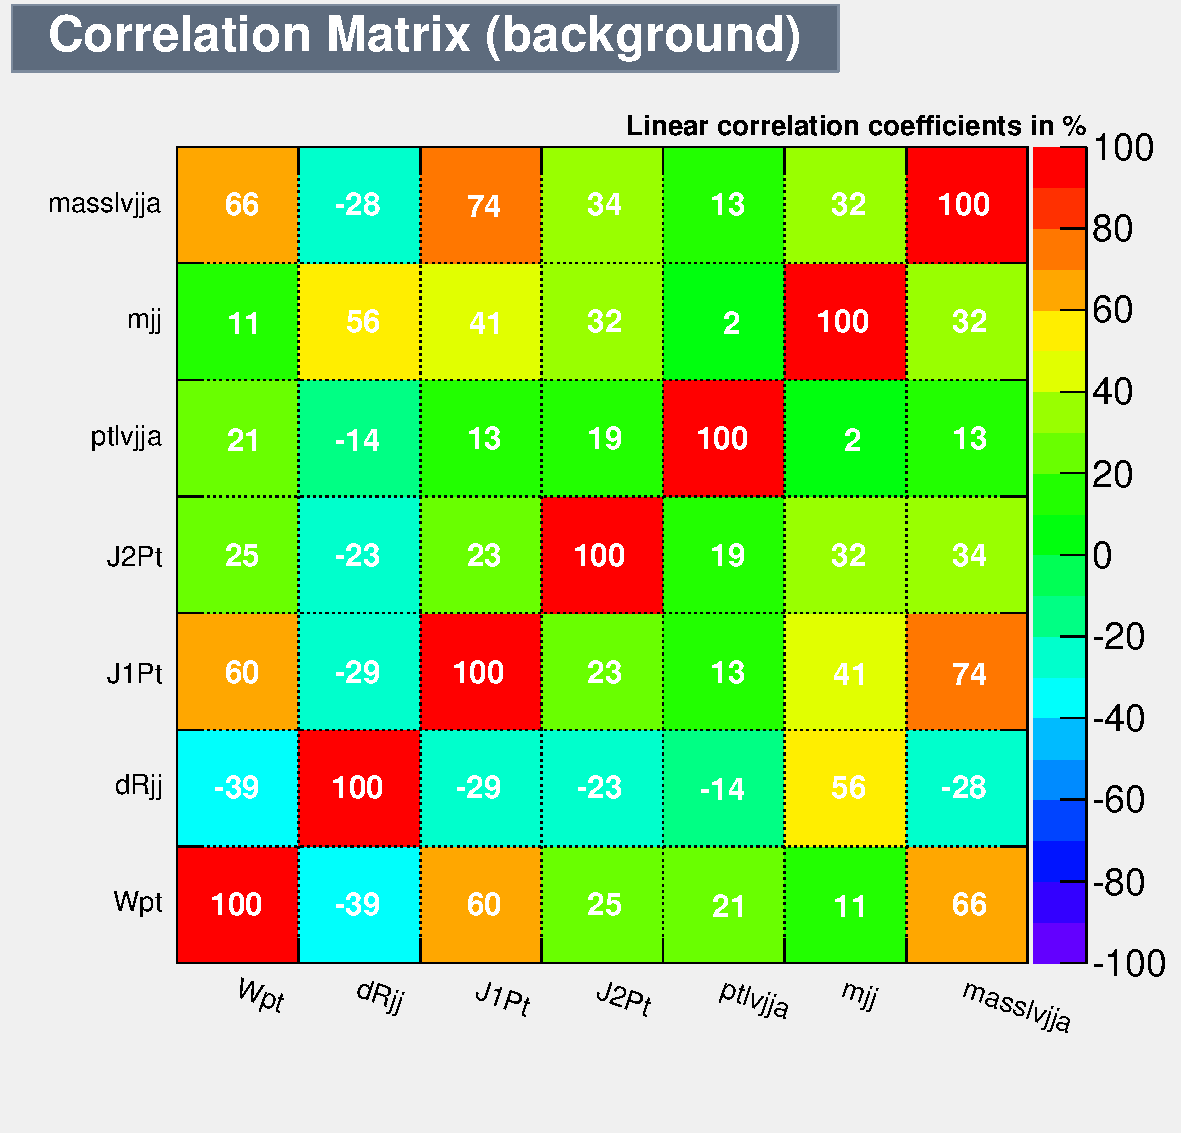
\includegraphics[width=0.4\textwidth]{figs/CorrelationMatrixB_SMWWA.pdf}
  }
    \caption{ The linear correlations between the input variables for signal and background for SM $WW\gamma$ muon channel. }
    \label{fig:corrSMmu}
  \end{center}
\end{figure}

The data-MC comparison for the SM $WW\gamma$ MVA output is shown on Figure ~\ref{fig:outSMmu}

\begin{figure}[]
  \begin{center}
    \subfigure[]{
    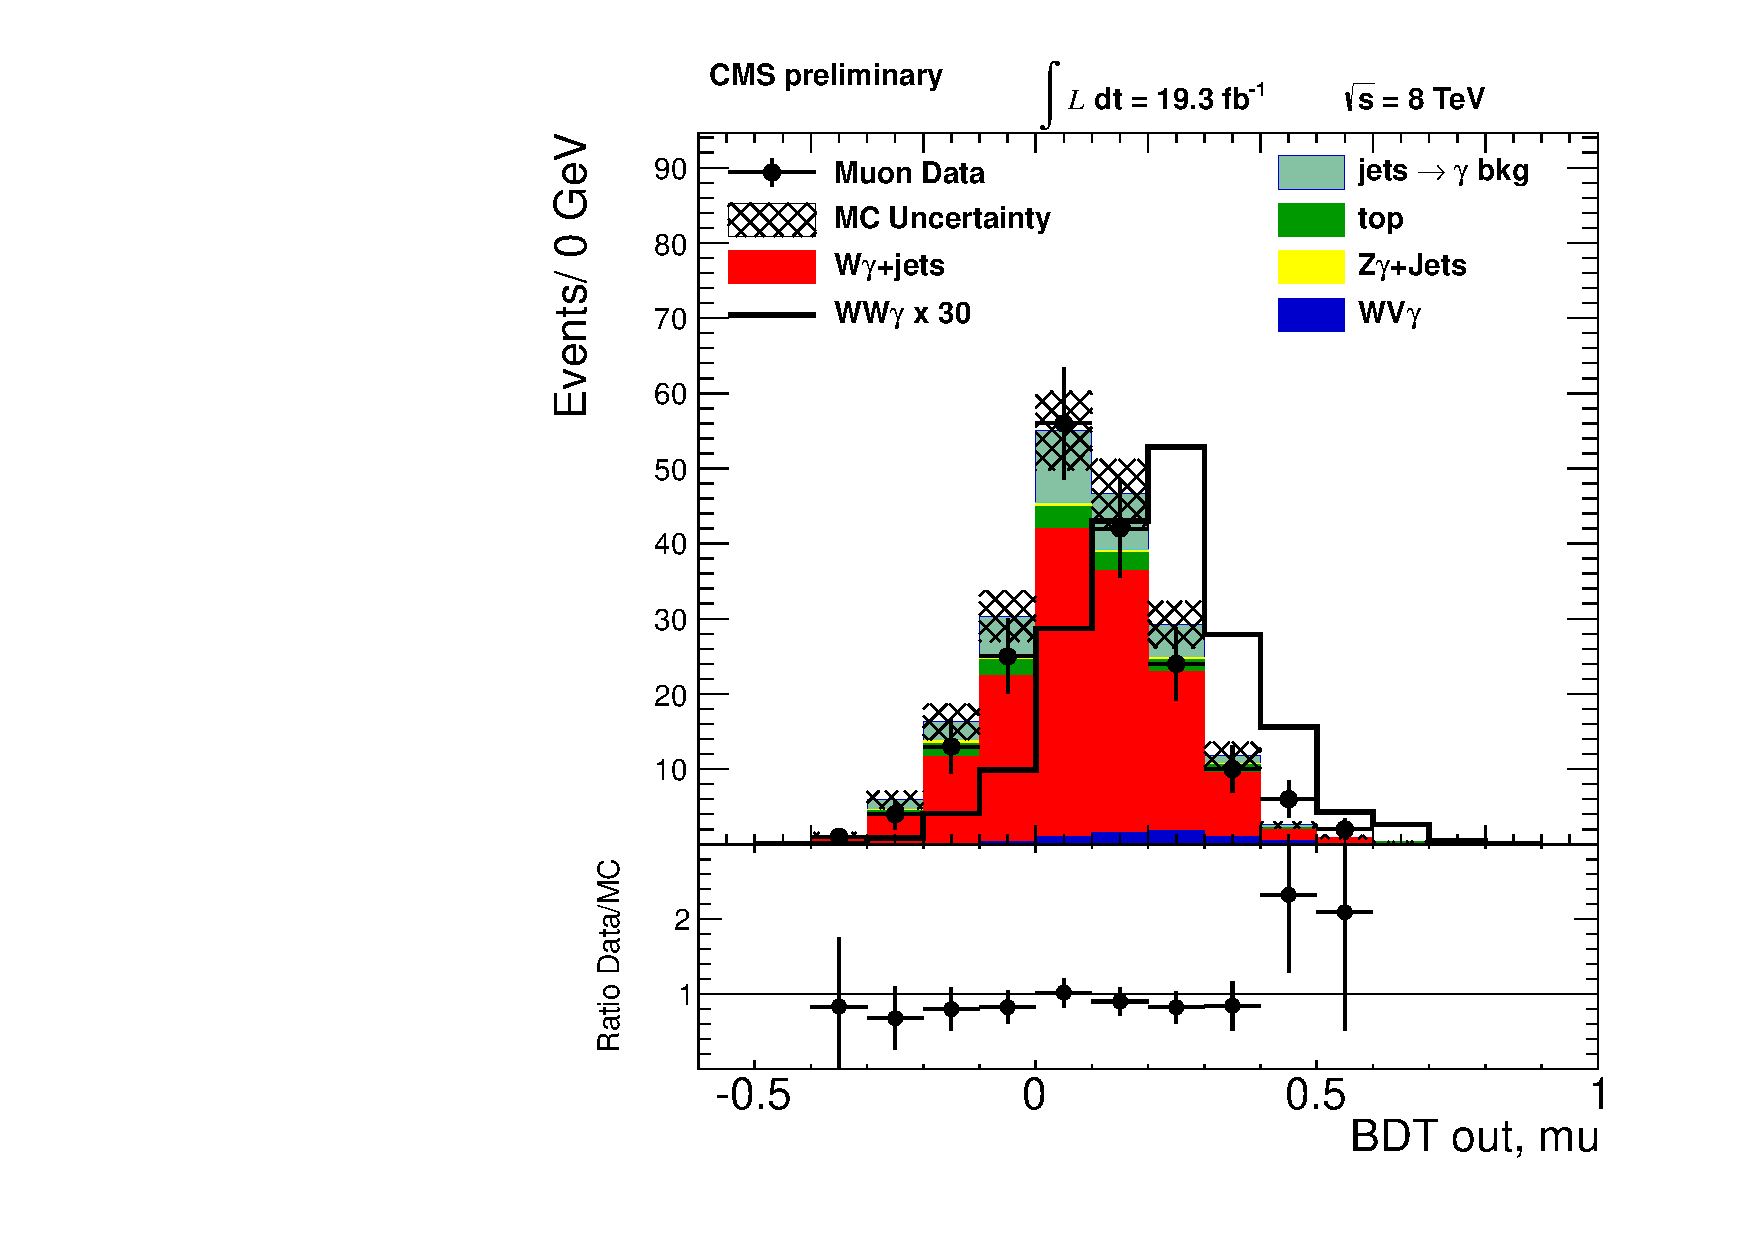
\includegraphics[width=0.4\textwidth]{figs/mu_mva2jWWAmuM.pdf}
  }
  \subfigure[]{
    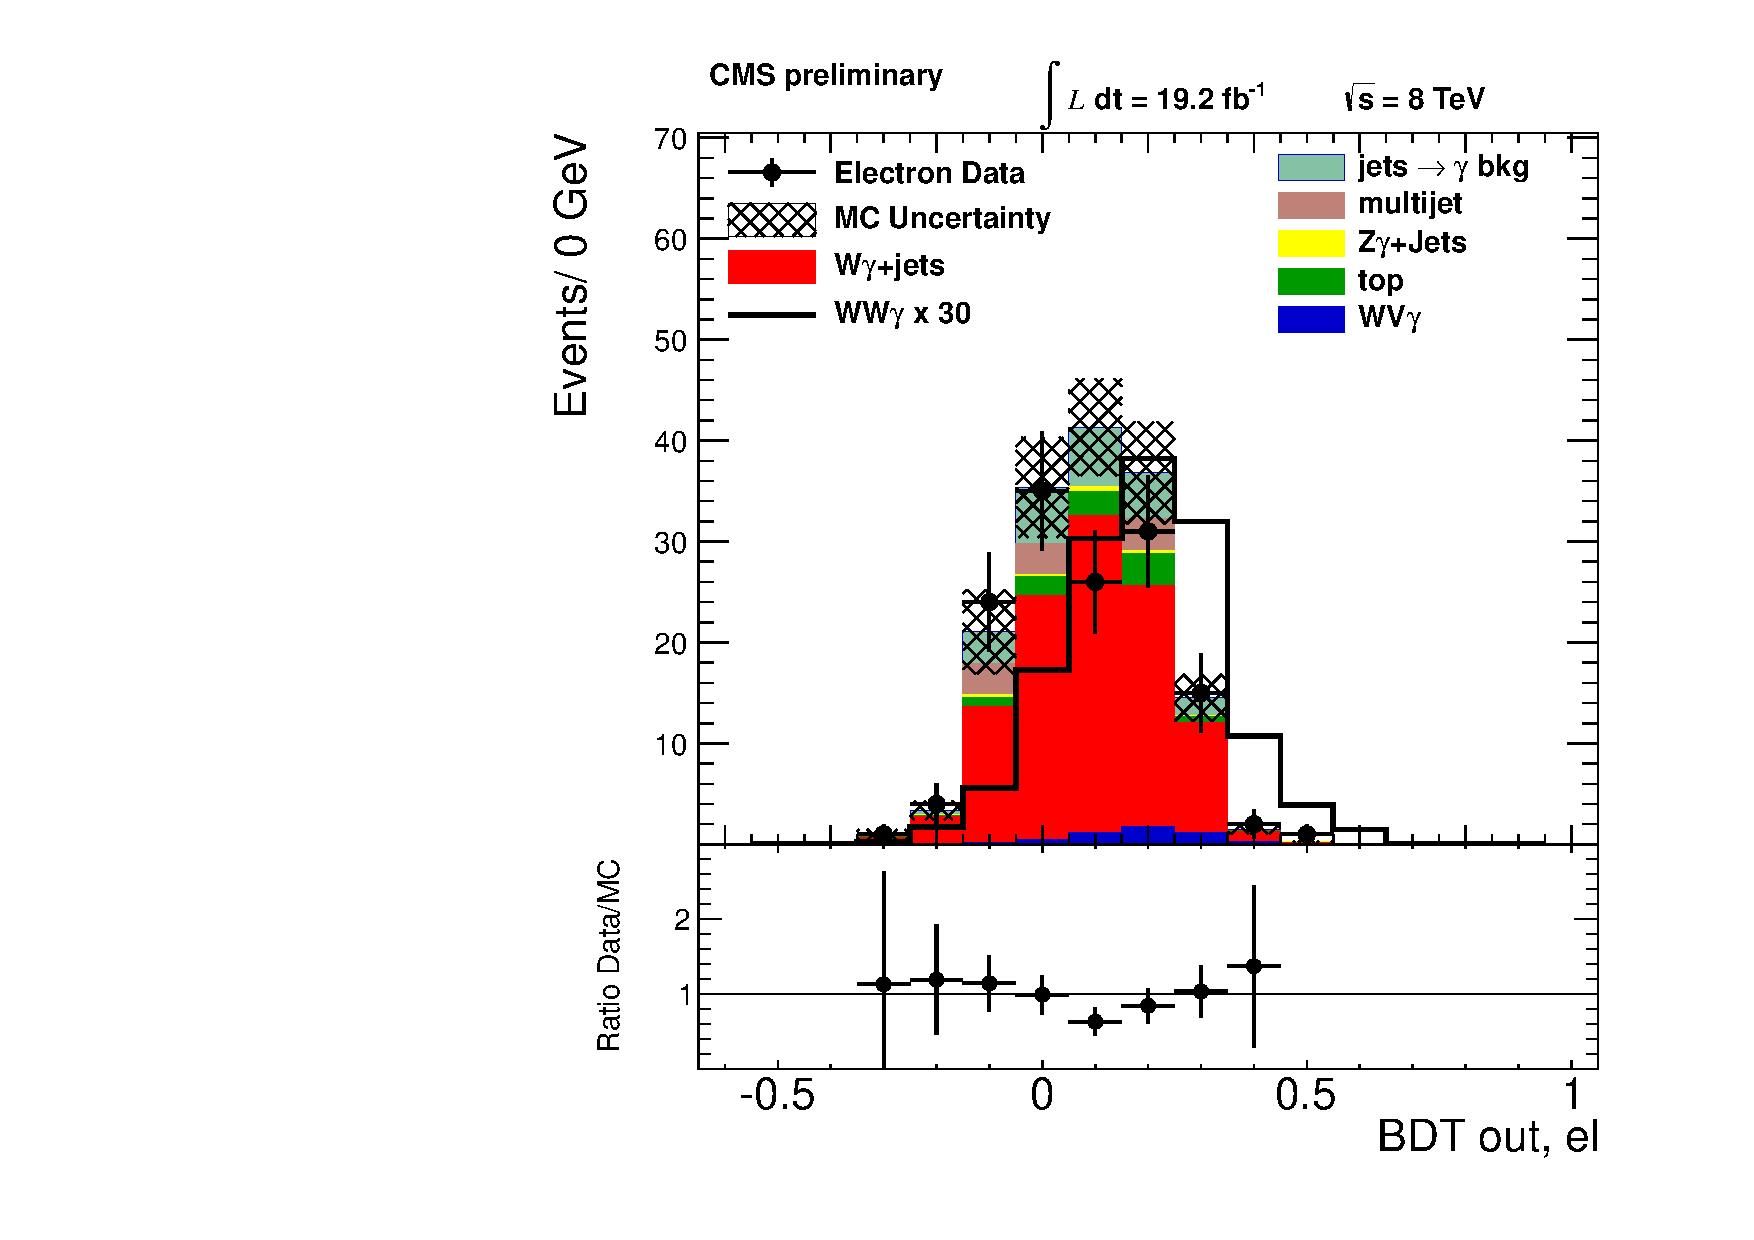
\includegraphics[width=0.4\textwidth]{figs/el_mva2jWWAelM.pdf}
  }
    \caption{ Data-MC comparison for the SM $WW\gamma$ MVA output of (a) muon and (b) electron channel. }
    \label{fig:outSMmu}
  \end{center}
\end{figure}

The signal efficiency vs the background rejection of the SM $WW\gamma$ BDT is shown in Figure~\ref{fig:rocSMmu} . The cut value on the MVA output is chosen in a 
way that it provides 80$\%$ signal efficiency and about 40$\%$ background rejections.

\begin{figure}[]
  \begin{center}
    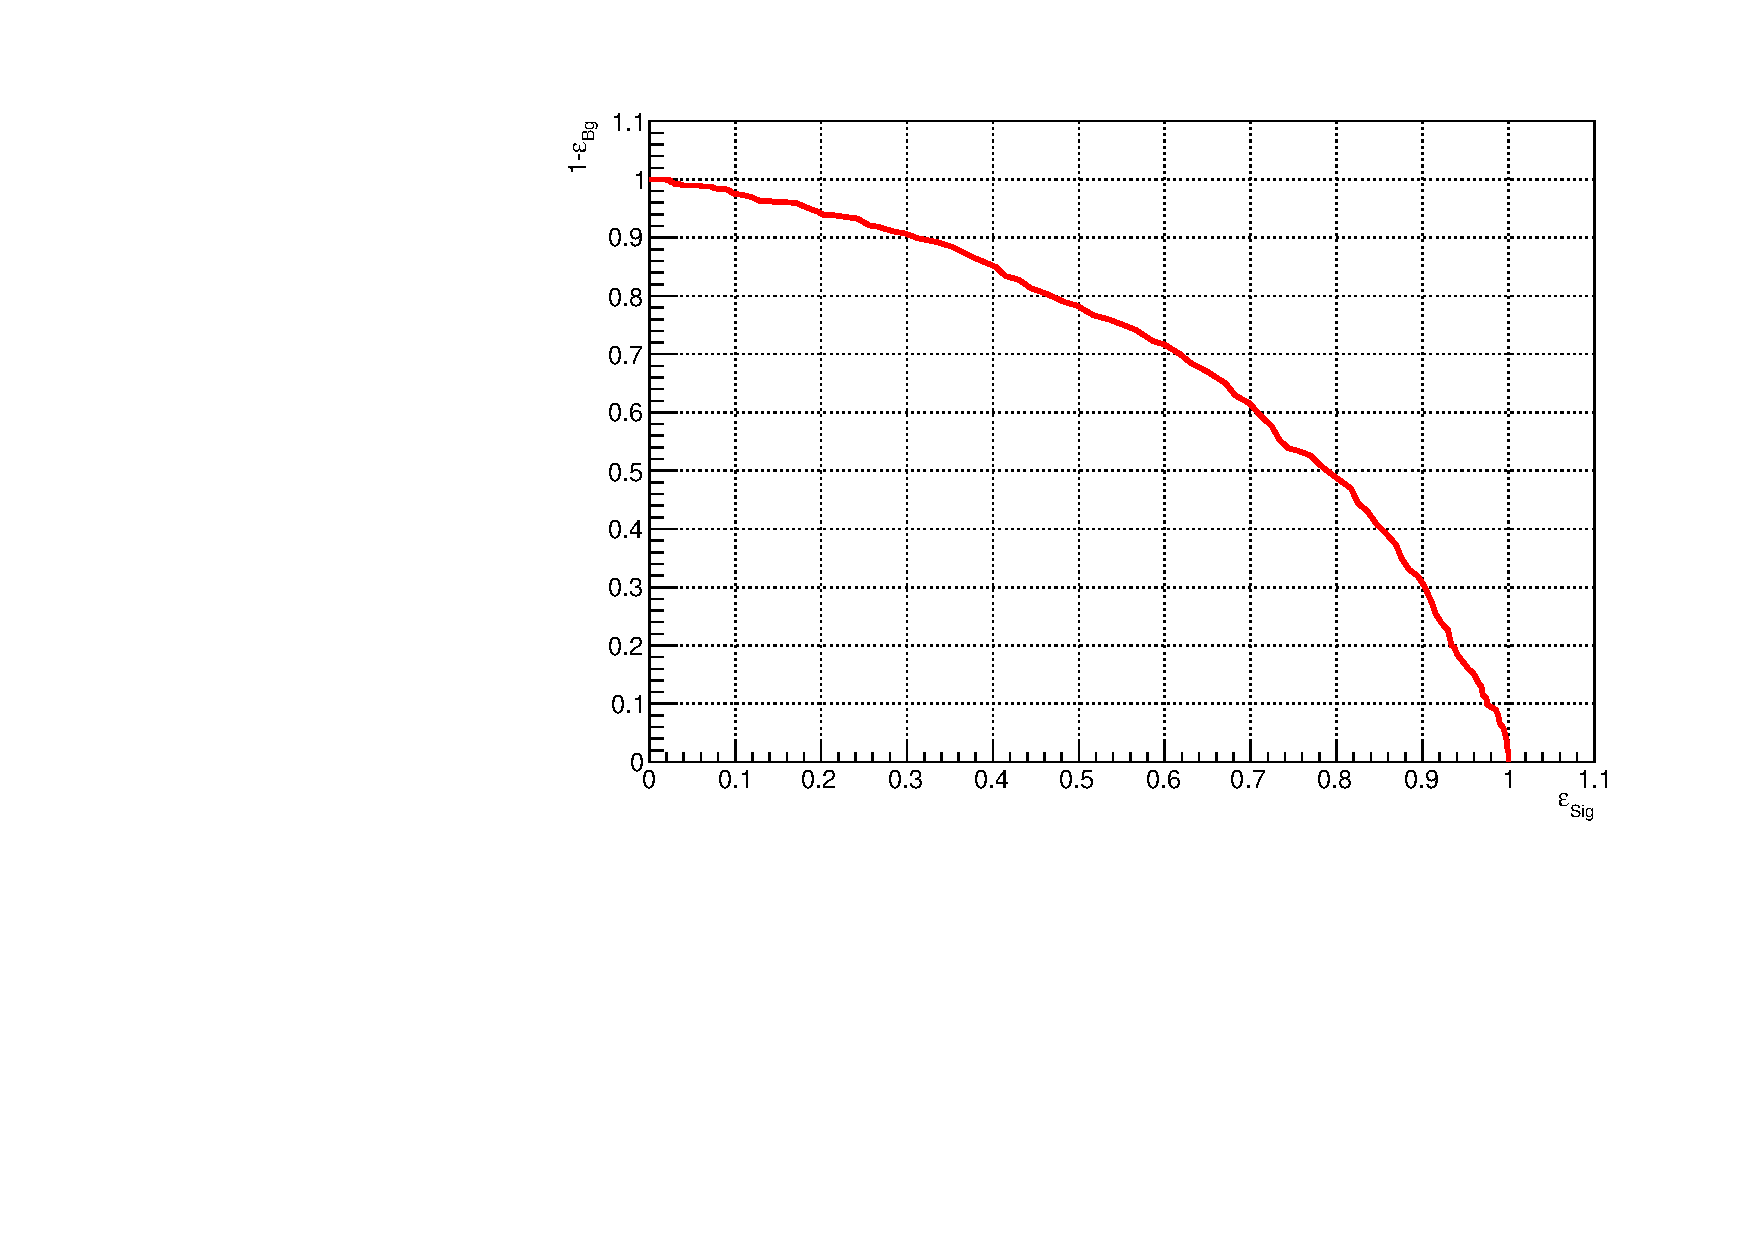
\includegraphics[width=0.4\textwidth]{figs/rocSM.pdf}
    \caption{ Signal efficiency vs the background rejection of the SM $WW\gamma$ BDT. }
    \label{fig:rocSMmu}
  \end{center}
\end{figure}

